\documentclass[11pt, letterpaper]{article}   	% use "amsart" instead of "article" for AMSLaTeX format
\usepackage{geometry}                		% See geometry.pdf to learn the layout options. There are lots.
\geometry{letterpaper}                   		% ... or a4paper or a5paper or ... 
%\geometry{landscape}                		% Activate for for rotated page geometry
%\usepackage[parfill]{parskip}    		% Activate to begin paragraphs with an empty line rather than an indent
\usepackage{graphicx}				% Use pdf, png, jpg, or es§ with pdflatex; use es in DVI mode
								% TeX will automatically convert es --> pdf in pdflatex		
\usepackage{amssymb}
\usepackage{amsmath}
%\usepackage{naaclhlt2013}
\usepackage{ mathtools}
\usepackage{cite}
\usepackage{multirow}
\usepackage{float}

\title{Alignment with Minimum Translation Units}
%\author{The Author}
%\date{}							% Activate to display a given date or no date

\begin{document}
\maketitle
\section{Task definition}
A sentence is a sequence of words $\textbf{w}=w_1 w_2 \cdots w_n $, where $w_i$ is the $i$-th word of the sentence. A phrase $s=w_i \cdots w_j $ is a contiguous subsequence of $\textbf{w}$. 
We mark the span covered by $s$ as $\bar{s}$, here $\bar{s}=[i,j]$.
\iffalse
\begin{equation}
\forall_{1\leqslant i \leqslant \textbf{f}} (\exists_{p\in seg} i \in p)  \wedge
\forall_{1\leqslant i \leqslant \textbf{f}} \forall_{p,p' \in seg} ({(i \in p \wedge i \in p') \rightarrow p=p'})
\end{equation}
\fi
Given a source sentence $\mathbf{f}$ with length $n$ and a target sentence $\mathbf{e}$ with length $m$, a phrasal alignment $A$ is a set of span pairs $A=\{(s,t) \, \mid \, \bigcup {s} = [1,n], \bigcap {s} = \emptyset,  \bigcup {t} = [1,m], \bigcap {t} = \emptyset \}$. Our task is to 
\begin{itemize} 
\item define a probabilistic model $p: \{\textbf{f} \times \textbf{e} \times A\} \rightarrow \mathbf{[0,1]}$
\item estimate the parameters in $p$
\item given $\textbf{f},\textbf{e}$, use some algorithm to find $\hat{A}=\operatorname*{argmax}_{A} p(\textbf{f} \times \textbf{e} \times A)$.
\end{itemize}
 
\section{Notation related to phrase}

\begin{itemize}
\item Span boundary: Given a span $\bar{s}=[i,j]$, we define its left boundary position as $\mathit{left}(\bar{s})=i$, right boundary position as $\mathit{right}(\bar{s})=j$. 

\item Phrase: Given a sentence $\textbf{f}=f_1 f_2 ... f_m$, and a span $[i,j]$, we can represent the phrase $f_i ... f_j$ as $\textbf{f}_{[i,j]}$
%\item Segmentation of span: $seg(s)=\{s' \mid s' \, \text{is a span}, \bigcup s' = s, \bigcap s' = \emptyset\}$
\end{itemize}

\section{Model $p$} 
We can define various models. Here we give some examples.
\begin{itemize}

\item Model 1:
\begin{enumerate}
\item generate a group of phrase pairs $\{(s,t)\}$
\item order the phrase pairs into sentence pairs
\end{enumerate}

The probability of tuple $(\textbf{f},\textbf{e},A)$ is 
\begin{equation} \label{eq:obj1}
p(\textbf{f},\textbf{e},A)=\prod_{(\bar{s},\bar{t})\in A}p(s,t)
\end{equation}

\item Model 1Coditional:
same as Model 1, except that we adopt conditional probability for phrase pair. $p(s,t)=p(t|s)p(s)$ and $p(s)=\prod_{w\in s} p(w)$ or in simplest case we set $p(s)=1$. What if we set the conditional probability to be summation of IBM model 1 probability? $p(t|s)=\prod_{w' \in t} \sum_{w\in s} p(w'|w)$. Then is the phrase-based model equivalent to IBM model 1? But what will happen after heavy pruning? like frequency based cutoff \cite{marcu-wong-02}, picking top $N$ $t$ for $s$.

\item Model 1Codintional*:
same as Model 1C, but with an additional component to generate source or target first. 
\begin{equation}
p(s,t)=p(\text{generate source})p(s)p(t|s)+p(\text{generate target})p(t)p(s|t)
\end{equation}. The motivation of adding this additional component is to use bi-directional word-based probability to do better pruning, otherwise $p(t|s)$ will bias long $s$ and short $t$.

\item Model 2:

\begin{enumerate}
\item generate begin of sentence pair $(\texttt{<s>},\texttt{<s>})$
\item generate phrase pair $(s,t)$, append $s$ to the end of generated partial source sentence
\item repeat step 2 step until end of sentence pairs $(\texttt{</s>},\texttt{</s>})$ was generated.
\item order the target phrases generated in step 2 into target sentence
\end{enumerate}

Let's assume the reordering follow a uniform distribution.
The probability of tuple $(\textbf{f},\textbf{e},A)$ is 
\begin{equation} \label{eq:obj2}
p(\textbf{f},\textbf{e},A))=\prod_{(\bar{s_i},\bar{t_i}) \in A} p((s_i,t_i)| (s_{i-1},t_{i-1}) ... (s_{1},t_{1}))
\end{equation}
where $left(\bar{s_i})- right(\bar{s_{i-1}})=1$

\iffalse
\item Model 3:
Same as model 2, but here we assume the reordering follow a slightly more complicated distribution than uniform.
\begin{equation} \label{eq:obj3}
f(\textbf{f},\textbf{e},A))=\prod_{(s_i,t_i) \in A} p((\bar{s_i},\bar{t_i})| (\bar{s_{i-1}},\bar{t_{i-1}}) ... (\bar{s_{1}},\bar{t_{1}})) p(d(i) | d(i-1) ... d(1)) )
\end{equation}
where $left(s_i)- right(s_{i-1})=1$, \quad $d(i)=left(t_i)- right(t_{i-1})$
\fi

\end{itemize}

\section{Parameter estimation}
\subsection{Basic Approach}
Given a sentence pair $(\textbf{f},\textbf{e})$, $p(\textbf{f},\textbf{e})=\sum_{A}p(\textbf{f},\textbf{e},A)$.\\
Given a parallel corpus $C$ where $A$ is the latent data, 
\begin{equation}p(C)=\prod_{(\textbf{f},\textbf{e}) \in C} p(\textbf{f},\textbf{e})=\prod_{(\textbf{f},\textbf{e}) \in C} \sum_{A} p(\textbf{f},\textbf{e},A) \end{equation}
We estimate the parameters by optimizing the objective function $p(C)$. EM is one of the ways to do the optimization with latent variables.

\subsection{Complexity}
Given a source sentence $S$ with length $n$, then we have number of phrases $\frac{n^2+n}{2}$ and number of segmentations $\sum\limits_{i=0}^{n-1} {n-1 \choose i} = 2^{n-1}$. (\cite{marcu-wong-02} claims the number is Stirling number of the second kind, which is the number of ways to select a subset of k elements from a set of n elements. I didn't find the proof.)

Given a source sentence $S$ with length $n$ and a target sentence $T$ with length $m$.  Let $n \leqslant m $, the number of possible phrasal alignments 
\begin{equation}
|\{A\}|= \sum \limits_{i=0}^{n-1} {n-1 \choose i}{m-1 \choose i}i!  > \sum \limits_{i=1}^{n-1} {n-1 \choose i}{n-1 \choose i} = {2n-2 \choose n-1} \sim \frac{4^n}{n^{1/2} \sqrt{\pi}}.
\end{equation}

Search for the best phrasal alignment is NP-Hard, sum over all alignments is PSPACE-hard \cite{denero-acl-08}.

%If the phrase segmentation of the source sentence is given, then this problem can be reduced to the longest path problem which is NP-complete.  So the original problem is NP-hard. 

\subsection{Pruning}
It's impractical to do parameter estimation and search in the original model space. Below are some heuristic ways to do pruning.
\begin{itemize}
\item filter out phrases appearing less than 5 times in the corpus, but keep all unigrams \cite{marcu-wong-02}
\item filter out phrases which is not compatible with word alignments. \cite{denero-06-wmt}
\end{itemize}

\subsection{Search Algorithm}
\begin{itemize}
\item Greedily hill climbing, with some heuristic actions : breaking and merging concepts, swapping words between concepts, and moving words across concept. \cite{marcu-wong-02}
\item Exponential-time dynamic programming with word alignment constraint.  \cite{denero-06-wmt}
\end{itemize}

\section{Analysis}
Why both of them underperform heuristic phrase extraction from word alignment?

\cite{marcu-wong-02} why?

\cite{denero-06-wmt} did not generate new phrases.

My guess is for M\textbf{e}, the decoding algorithm and LM are so powerful that the probability of phrase pair doesn't matter a lot. And the content of phrase pairs matter more. The phrasal alignment approaches don't necessarily generate more correct phrase pairs than the heuristic way.

\subsection{Pilot experiment}
If the guess above is correct, then the contribution from EM will not be significant. Initialization will be good enough. To test it, we just use the phrase table estimated from the initialization step for decoding. And compare the performance with state-of-the-art phrase table extraction. 

\subsubsection{Setting}
\begin{itemize}
\item Training Data: first 100k lines of corev5
\item Dev Data: corev5.6 tune
\item Test Data: corev5.6 test
\item Language model: trigram language model trained on GIGAWORD3.
\item System: Moses \cite{moses-07}
\end{itemize}

\subsubsection{Phrase pairs extraction approaches}
We try and compare following different approaches.

\begin{enumerate}
\item \label{app1} Approach in \cite{marcu-wong-02}. Filter out phrases appearing less than 5 times in the corpus\footnote{It's interesting to see how the cutoff value will impact the number of phrases of different length.}, but keep all unigrams, attach t-distribution score to them.
Suppose we have sentence pair$(s,t)$, phrase pair $(p_s,p_t), |s|=n, |t|=m,|p_s|=k,|p_t|=l$, the t score for this phrase pair is $\frac{|\{A \,of \,(s,t) \mid \,\text{fixing}\, (p_s,p_t)\}|}{|\{A\,of \,(s,t)\}|}$

\begin{equation}
\begin{cases}
\frac
{\sum \limits_{i=0}^{min(n-k-1,m-l-1)} {n-k-1 \choose i}{m-l-1 \choose i}(i+2)! }
{\sum \limits_{i=0}^{min(n-1,m-1)} {n-1 \choose i}{m-1 \choose i}(i+1)! }  & \text{if both $p_s, p_t$ are at the boundary} \\
\frac
{\sum \limits_{i=0}^{min(n-k-2,m-l-2)} {n-k-2 \choose i}{m-l-2 \choose i}(i+3)! }
{\sum \limits_{i=0}^{min(n-1,m-1)} {n-1 \choose i}{m-1 \choose i}(i+1)! }  & \text{if both $p_s,p_t$ are in the middle} \\
\frac
{\sum \limits_{i=0}^{min(n-k-1,m-l-2)} {n-k-1 \choose i+1}{m-l-2 \choose i}(i+3)! }
{\sum \limits_{i=0}^{min(n-1,m-1)} {n-1 \choose i}{m-1 \choose i}(i+1)! }  & \text{if $p_s$ is at the boundary, $p_t$ is in the middle} \\
\frac
{\sum \limits_{i=0}^{min(n-k-2,m-l-1)} {n-k-2 \choose i}{m-l-1 \choose i+1}(i+3)! }
{\sum \limits_{i=0}^{min(n-1,m-1)} {n-1 \choose i}{m-1 \choose i}(i+1)! }  & \text{if $p_t$ is at the boundary, $p_s$ is in the middle} \\
\end{cases}
\end{equation}. 
Because $|A|$ overestimate the number of true alignments, and the ratio of overestimation is exponential to the length of sentence, theoretically we should multiply it with an exponential penalty $\alpha^n$ where $0<\alpha<1$. As a effect, it is equivalent to multiply the numerator with $\frac{1}{\alpha^{min(k,l)}}$. But we don't know what's a good value for $\alpha$, for simplicity, we choose to overestimate the numerator by letting it be ${\sum \limits_{i=0}^{min(n-k-1,m-l-1)} {n-k-1 \choose i}{m-l-1 \choose i}(i+2)! }$ for all the different cases. After training, \cite{marcu-wong-02} normalize the joint probability to conditional probability( 2 directions: source to target, target to source).

\item \label{app1c} Use Model 1C with constraint 0 $<$ phrase length $< X$, attach IBM model 1 score (2 directions) for each phrase pair. How to choose the X? (State-of-the-art MT system Moses\cite{moses-07} sets the maximal phrase length to be 7. )

\begin{enumerate}

\item Compare with and without IBM model 1 score
\begin{table}[H]
\centering
\begin{tabular}{| c | c| }
\hline
\bf{pure marcu and wong} & \bf{+ IBM model 1 scores}\\
\hline
12.4 & 17.6\\
\hline
\end{tabular}
\label{tab:BLEUibmfeature}
\caption{BLEU of with and without IBM model1 score, max phrase length=7, phrase count cutoff=5 }
\end{table}

\textbf{Discussion:} IBM model 1 scores help improve 5 BLEU points. This suggests that feature values matter.

\item Compare different max phrase length and cutoff%, and Top N target phrases selection

\begin{table}[H]
\centering
\begin{tabular}{ c c | c | c | c | c|c }
& \multicolumn{5}{c}{\bf{ count cutoff}}  \\
&  & 1 &	2 &	3 &	4 &	5\\
\hline
\multirow{7}{*}{\bf{max length}}
& 1 &	11.9 &	11.9 &	11.9 &	11.9 &	11.9\\
\cline{2-7}
& 2 &	16.4 &	16.2 &	16.2 &	15.7 &	15.6\\
\cline{2-7}
& 3 &	16.9 &	17.2 &	16.6 &	17.1 &	17\\
\cline{2-7}
& 4 &	17.5 &	17.6 &	17.5 &	17.2 &	17.5\\
\cline{2-7}
& 5 &	17.9 &	18 &	17.5 &	17.6 &	17.7\\
\cline{2-7}
& 6 &	17.6 &	17.8 &	17.5 &	17.7 &	17.8\\
\cline{2-7}
& 7 &	17.9 &	17.9 &	17.6 &	18 &	17.6\\
\hline
\end{tabular}
\label{tab:fraclex}
\caption{BLEU of different maxlen and cutoff , keep all target phrases}
\end{table}

\textbf{Discussion:}
\begin{itemize}
\item Generally, the smaller cutoff the better, the longer phrases the better
\item Max length longer than 5 don't show significant improvement
\end{itemize}

\item Use Fractional count only, \textbf{NO} IBM model 1 score
\begin{table}[H]
\centering
\begin{tabular}{ c c | c | c | c | c|c }
& \multicolumn{5}{c}{\bf{ count cutoff}}  \\
&  & 1 &	2 &	3 &	4 &	5\\
\hline
\multirow{7}{*}{\bf{max length}}
& 1 &	9.14 &	9.14 &	9.14 &	9.14 &	9.14\\
\cline{2-7}
& 2 &	11.8 &	10 &	11.9 &	11.8 &	12.2\\
\cline{2-7}
& 3 &	11.1 &	11.7 &	11.8 &	12.5 &	12.4\\
\cline{2-7}
& 4 &	11.5 &	8.72 &	11.9 &	11.1 &	12.4\\
\cline{2-7}
& 5 &	11.4 &	11.6 &	11.9 &	12.4 &	12\\
\cline{2-7}
& 6 &	11.8 &	11.7 &	11.6 &	11 &	11.2\\
\cline{2-7}
& 7 &	11.6 &	11.5 &	12.2 &	12 &	12.4\\
\hline
\end{tabular}
\label{tab:fraconly}
\caption{BLEU of different maxlen and cutoff , keep all target phrases}
\end{table}

\item Use absolute count of each phrase pairs and renormalize, keep IBM model 1 scores
\begin{table}[H]
\centering
\begin{tabular}{ c c | c | c | c | c|c }
& \multicolumn{5}{c}{\bf{ count cutoff}}  \\
&  & 1 &	2 &	3 &	4 &	5\\
\hline
\multirow{7}{*}{\bf{max length}}
& 1 &	11.8 &	11.8 &	11.8 &	11.8 &	11.8\\
\cline{2-7}
& 2 &	15.8 &	15.6 &	16.1 &	15.5 &	15.7\\
\cline{2-7}
& 3 &	17.3 &	17 &	17 &	17.3 &	16.5\\
\cline{2-7}
& 4 &	17.9 &	17.6 &	17.5 &	17.5 &	17.5\\
\cline{2-7}
& 5 &	17.9 &	18 &	17.5 &	17.6 &	17.6\\
\cline{2-7}
& 6 &	17.9 &	17.8 &	17.5 &	17.7 &	17.8\\
\cline{2-7}
& 7 &	18.1 &	17.9 &	17.6 &	18 &	17.6\\
\hline
\end{tabular}
\label{tab:countlex}
\caption{BLEU of different maxlen and cutoff , using absolute count for phrase pairs, keep all target phrases}
\end{table}

\item Use absolute count of each phrase pairs and renormalize, \textbf{NO} IBM model 1 scores
\begin{table}[H]
\centering
\begin{tabular}{ c c | c | c | c | c|c }
& \multicolumn{5}{c}{\bf{ count cutoff}}  \\
&  & 1 &	2 &	3 &	4 &	5\\
\hline
\multirow{7}{*}{\bf{max length}}
& 1 &	9.51 &	9.51 &	9.51 &	9.51 &	9.51\\
\cline{2-7}
& 2 &	11.3 &	12 &	12.2 &	8.57 &	12.4\\
\cline{2-7}
& 3 &	11.8 &	11.7 &	7.97 &	12 &	12.6\\
\cline{2-7}
& 4 &	11.4 &	11.9 &	12.1 &	12.1 &	11.9\\
\cline{2-7}
& 5 &	11.5 &	11.8 &	8.67 &	12.1 &	12\\
\cline{2-7}
& 6 &	11.8 &	\bf{N.A.} &	12 &	11.7 &	12.6\\
\cline{2-7}
& 7 &	7.95 &	11.8 &	12.3 &	12 &	12.7\\
\hline
\end{tabular}
\label{tab:countonly}
\caption{BLEU of different maxlen and cutoff , keep all target phrases}
\end{table}

\item Using IBM model 1 scores only

\begin{table}[H]
\centering
\begin{tabular}{ c c | c | c | c | c|c }
& \multicolumn{5}{c}{\bf{ count cutoff}}  \\
&  & 1 &	2 &	3 &	4 &	5\\
\hline
\multirow{7}{*}{\bf{max length}}
& 1 &	11.6 &	11.6 &	11.6 &	11.6 &	11.6\\
\cline{2-7}
& 2 &	14.2 &	14.9 &	15.1 &	14.9 &	15\\
\cline{2-7}
& 3 &	15.6 &	15.8 &	15.6 &	15.6 &	15.6\\
\cline{2-7}
& 4 &	16.8 &	16.3 &	16.2 &	15.6 &	16.1\\
\cline{2-7}
& 5 &	16.1 &	16.4 &	16.7 &	16.2 &	16.3\\
\cline{2-7}
& 6 &	15.5 &	16.6 &	16.6 &	16.1 &	16.4\\
\cline{2-7}
& 7 &	16.2 &	16.4 &	16.5 &	16.6 &	16\\
\hline
\end{tabular}

\label{tab:lexonly}
\caption{BLEU of different maxlen and cutoff }
\end{table}
\end {enumerate}

\item \label{app3} State-of-the-art heuristic phrase extraction: run GIZA++($1^52^5H^53^34^3$), compute the viterbi alignment for source-to-target and target-to-source directions, use heuristic grow-diag-final to combine the two alignments. Extract the phrases according to the alignment constraint. For each phrase pair, compute phrasal and lexical conditional probabilities for source-to-target and target-to-source directions.

\begin{table}[H]
\centering
\begin{tabular}{|c | c | c| c| c| }
\hline
\bf{Feature set} & \bf{Standard} & \bf{No Lex} &\bf{Only Lex} & \bf {Only Lex by IBM model1}\\
\hline
\bf{BLEU} & 19.4 & 19.2 & 18.5 & 18.6\\
\hline
\end{tabular}
\label{tab:BLEUStandard}
\caption{BLEU vs different  feature set }
\end{table}

\textbf{Discussion:} Comparing table \ref{tab:lexonly} and table \ref{tab:BLEUStandard} , we can see by filtering out some redundant phrase pairs, we can have 18.6-16.8=1.8 BLEU improvement

\item Keep top N target phrases according to the sum of bi-directional IBM model 1 score. (Use bidirectional conditional probability by fractional counts and IBM model 1 scores as features for decoding).
\begin{enumerate}
\item N=100
\begin{table}[H]
\centering
\begin{tabular}{ c c | c | c | c | c|c }
& \multicolumn{5}{c}{\bf{ count cutoff}}  \\
&  & 1 &	2 &	3 &	4 &	5\\
\hline
\multirow{7}{*}{\bf{max length}}
& 1 &	12 &	12 &	12 &	12 &	12\\
\cline{2-7}
& 2 &	16.3 &	15.9 &	16.2 &	15.9 &	16.1\\
\cline{2-7}
& 3 &	\bf{N.A.} &	16.9 &	17.1 &	16.4 &	16.7\\
\cline{2-7}
& 4 &	\bf{N.A.} &	\bf{N.A.} &	16.9 &	16.9 &	16.9\\
\cline{2-7}
& 5 &	17 &	16.8 &	17 &	17 &	17.2\\
\cline{2-7}
& 6 &	17.3 &	17 &	17.2 &	17.1 &	16.8\\
\cline{2-7}
& 7 &	\bf{N.A.} &	17 &	17 &	16.8 &	16.8\\
\hline
\end{tabular}
\label{tab:top100}
\caption{BLEU of different maxlen and cutoff, keep top 100 target phrases}
\end{table}

\item N=1000
\begin{table}[H]
\centering
\begin{tabular}{ c c | c | c | c | c|c }
& \multicolumn{5}{c}{\bf{ count cutoff}}  \\
&  & 1 &	2 &	3 &	4 &	5\\
\hline
\multirow{7}{*}{\bf{max length}}
& 1 &	11.9 &	11.9 &	11.9 &	11.9 &	11.9\\
\cline{2-7}
& 2 &	15.8 &	15.9 &	16.4 &	16.2 &	15.8\\
\cline{2-7}
& 3 &	\bf{N.A.} &	17.2 &	16.9 &	16.4 &	16.4\\
\cline{2-7}
& 4 &	17.4 &	17.4 &	17.3 &	17 &	16.9\\
\cline{2-7}
& 5 &	17.6 &	17.5 &	17.2 &	17.5 &	17.1\\
\cline{2-7}
& 6 &	17.8 &	17.7 &	17.5 &	17.6 &	17.2\\
\cline{2-7}
& 7 &	17.5 &	17.7 &	17.3 &	17.4 &	17.5\\
\hline
\end{tabular}
\caption{BLEU of different maxlen and cutoff, keep top 1000 target phrases}
\end{table}
\end{enumerate}
\textbf{Discussion:} keeping top 1000 target phrases still hurts the performance a little bit. We may need a better metric to help us do selection

\end{enumerate}

\subsubsection{Relaxed Task: Phrasal IBM Model 1}
Given a source sentence $\mathbf{f}$ with length $n$ and a target sentence $\mathbf{e}$ with length $m$, a phrasal alignment $A$ is a set of span pairs $A=\{(\bar{s},\bar{t}) \, \mid \, \bigcup {\bar{t}} = [1,m], \bigcap {\bar{t}} = \emptyset,  \bigcup{\bar{s}} \subseteq [1,n] \}$.
\begin{itemize}
\item Phrasal IBM Model 1
\begin{enumerate}
\item iteratively select a phrase in $\mathbf{f}$ to generate a target phrase
\item order the target phrases into sentence $\mathbf{e}$
\item The probability of pair $(\textbf{e},A)$ given $\textbf{f}$ is 
\begin{equation} \label{eq:obj1}
p(\textbf{e},A|\textbf{f})=\prod_{(\bar{s},\bar{t})\in A}p(t|s)
\end{equation}
\end{enumerate}

\item Expectation count computation: Given a sentence, expected count of a phrase pair
\begin{equation}
frac(s,t)=\frac{\sum_{A \, | \,(\bar{s},\bar{t})\in A} p(\textbf{e},A|\textbf{f})}{\sum_{A} p(\textbf{e},A|\textbf{f})}
\end{equation}
Let's denote the source part of the alignment $A$ as $S(A)=\{\bar{s}|(\bar{s},\bar{t})\in A\}$. The target part of the alignment as $T(A)=\{\bar{t}|(\bar{s},\bar{t})\in A\}$. In the relaxed task, that $T(A)$ is a segmentation of the target sentence, while $S(A)$ is not necessary a segmentation of the source sentence. Let's denote $G$ a segmentation of the target sentence, we have
 
\begin{align}
\sum_{A} p(\textbf{e},A|\textbf{f})=&\sum_{A} \prod_{(\bar{s},\bar{t})\in A} p(t|s)\\
=&\sum_{G} \sum_{A|T(A)=G} \prod_{(\bar{s},\bar{t})\in A} p(t|s)
\end{align}

We can denote the part after the $\sum_{G}$ symbol in the above equation as $p(\textbf{e},G | \textbf{f})$, which means the probability of the target sentence being generated with segmentation $G$, i.e. every phrase by the segmentation $G$ is an atom unit being generated. Fortunately, $p(\textbf{e},G | \textbf{f})$ can be computed efficiently by applying commutative property of multiplication and dynamic programming.

\begin{align}
p(\textbf{e},G | \textbf{f})=&\sum_{A|T(A)=G} \prod_{(\bar{s},\bar{t})\in A} p(t|s)\\
=& \prod_{\bar{t}\in G} \sum_{s|\bar{s} \subseteq [1,n]} p(t|s)
\end{align}
We can denote the probability of a target phrase generated as an atom unit as $p(t,\bar{t}|\textbf{f})=\sum_{s|\bar{s} \subseteq [1,n]}p(t|s)$. The complexity of computing this is equal to the number of source phrases. This can be computed in time $O(nd)$, where d is the maximal phrase length. There are also $O(nd)$ target phrases, so in total, we need $O(n^2d^2)$ time to compute $p(t,\bar{t}|\textbf{f})$ for all the $t$. With the computed target phrase probability, we can compute the probability for a segmentation $G$ in $O(n)$ time.

To compute $p(\textbf{e}|\textbf{f})=\sum_{G}p(\textbf{e},G | \textbf{f})$, which is the summation of all possible segmentation prob, we can use dynamic programming. Let's denote $p(\textbf{e}_{[1,j]}|\textbf{f})$ as the probability of generating the target words covering span $[1,j]$. We have
\begin{equation}
p(\textbf{e}_{[1,j]}|\textbf{f})=\sum \limits_{k=1}^d p(\textbf{e}_{[1,j-k]}|\textbf{f})p(\textbf{e}_{[j-k+1,j]},[j-k+1,j]|\textbf{f})
\end{equation}
This takes $O(n)$ time.

We can also compute $p(\textbf{e}_{[j,m]}|\textbf{f})$ similarly in $O(n)$  from backward.
Then we can compute expected count of a phrase pair $(s,t)$ where $t=\textbf{e}_{[i,j]}$, $s$ is any source phrase.
\begin{align}
frac(s,t)=&\frac{\sum_{A \, | \,(\bar{s},\bar{t})\in A} p(\textbf{e},A|\textbf{f})}{\sum_{A} p(\textbf{e},A|\textbf{f})}\\
=& \frac{p(\textbf{e}_{[1,i-1]}|\textbf{f})p(\textbf{e}_{[i,j]}|s)p(\textbf{e}_{[j+1,m]}|\textbf{f}) }    {p(\textbf{e}|\textbf{f})}
\end{align}


\end{itemize}


\subsubsection{Phrase Count Statistics}
\textbf{NOTE:} numbers in this subsection are based on the whole core data, need to be updated
\begin{itemize}
\item For the Approach in \cite{marcu-wong-02},
Questions: 1. how many phrases will appear more than 5/X times? And what's the average length of such phrases? 

\begin{table}[H]
\centering
\begin{tabular}{ c | c | c | c | c }
 & \multicolumn{2}{c}{\bf{Chinese}} & \multicolumn{2}{|c}{\bf{English}}  \\
  \cline{2-5} 
  \bf{cutoff} & \bf{\#phrases} & \bf{avg. length} & \bf{\#phrases} & \bf{avg. length} \\
  \hline
  1 & $5.07 \times 10^7$  & $6.40$ & $6.57\times 10^7$ & $6.69$  \\
  \hline
  2 & $5.42\times 10^6$ & $5.07$ &$5.78\times 10^6$ & $5.02$\\
  \hline
  3 & $1.86\times 10^6$  & $4.11$ & $2.31\times 10^6$& $4.30$\\
  \hline
  4 & $1.04\times 10^6$ & $3.58$ &$1.36\times 10^6$ &$3.86$\\
 \hline
  5 & $0.72\times 10^6$ & $3.31$ & $0.97\times 10^6$&$3.65$\\
  \hline
 \end{tabular}
 \caption{cutoff frequency vs phrase table size}
  \label{tab:phrase-cutoff}
\end{table}

\begin{figure}[p]
\centering
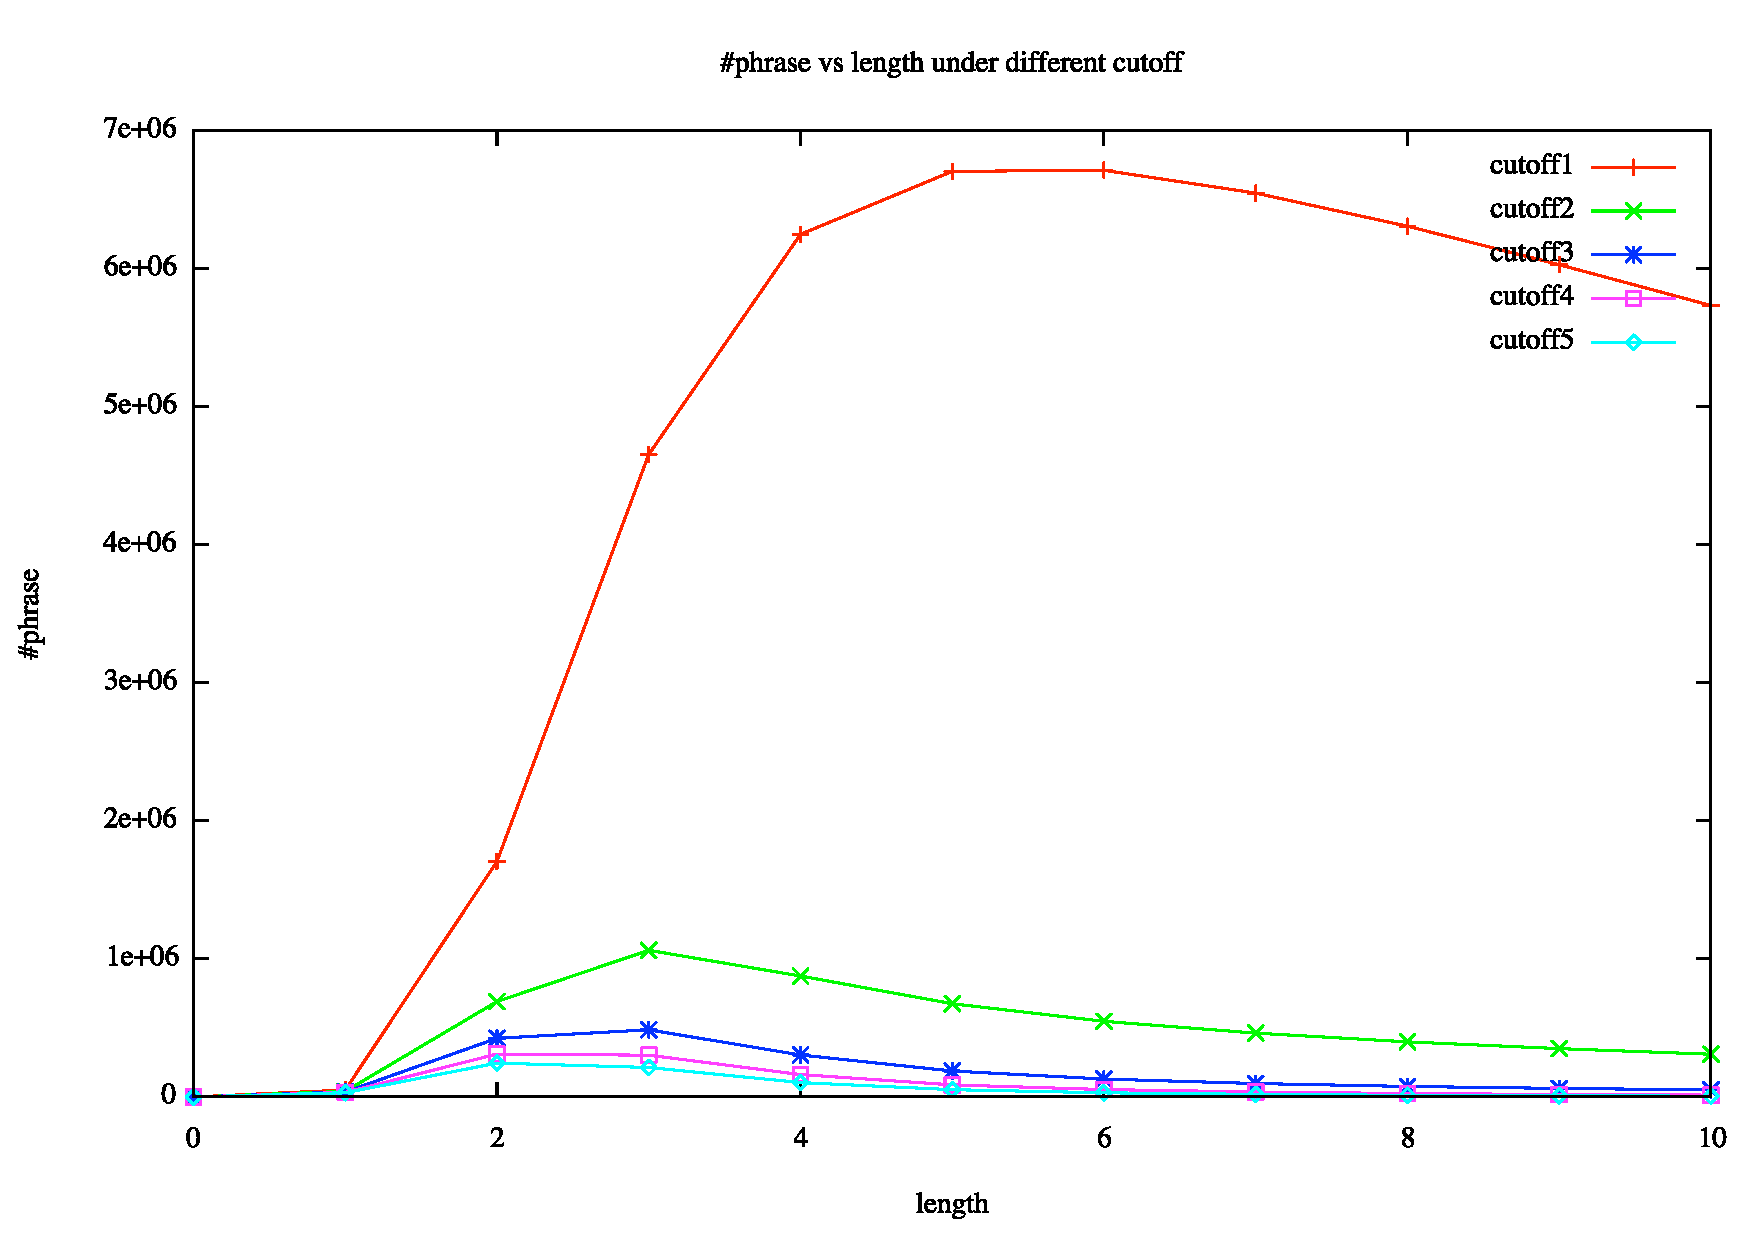
\includegraphics[width=1.0\textwidth]{phrase-count-chinese.pdf}
\caption{phrase count vs cutoff: Chinese}
\label{fig:phrase-count-chinese}
\end{figure}

\begin{figure}[p]
\centering
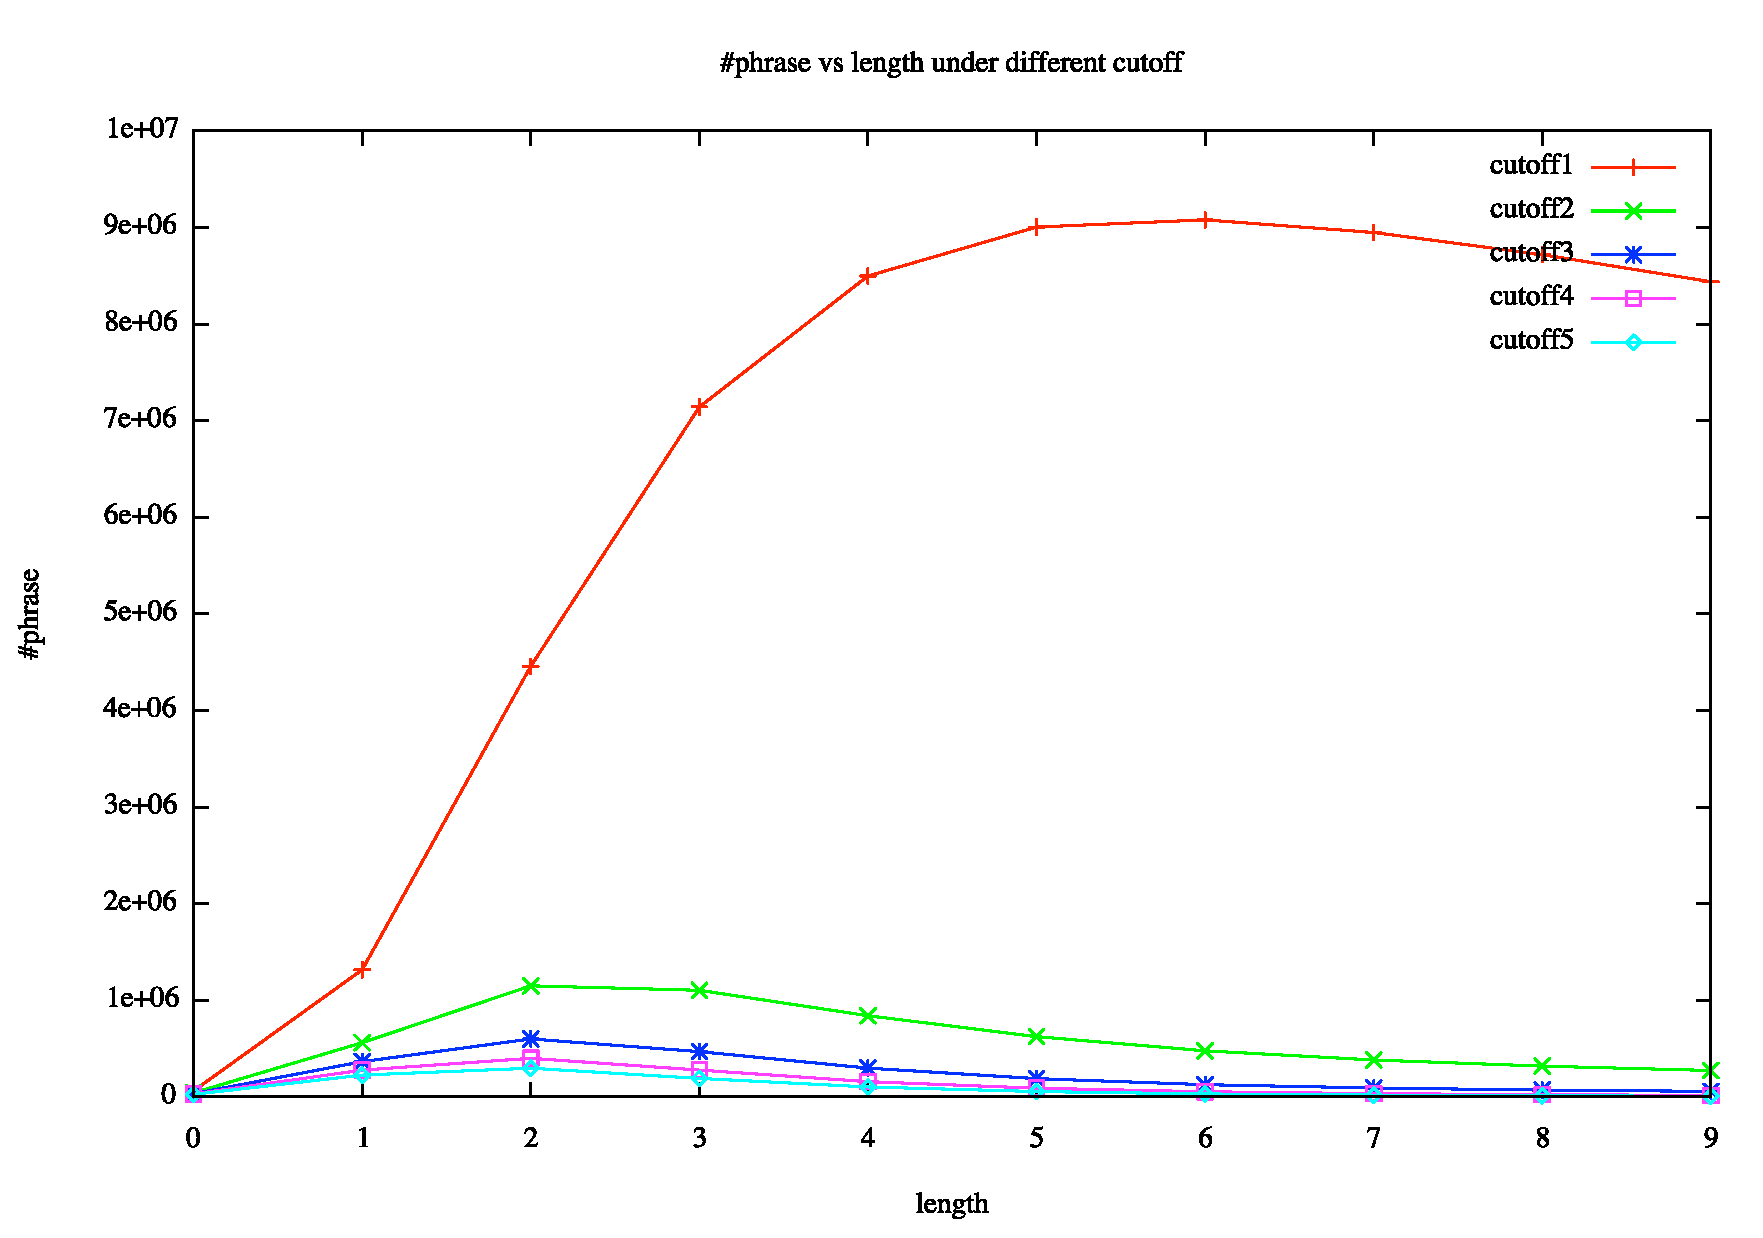
\includegraphics[width=1.0\textwidth]{phrase-count-english.pdf}
\caption{phrase count vs cutoff: English}
\label{fig:phrase-count-english}
\end{figure}

\item For State-of-the-art heuristic phrase extraction, 
\begin{itemize}
\item try blocking the phrase conditional probability. 
Problem encountered: mert script offers some options to set value range for any feature. I set the value range for phrase conditional probability to [0,0]. However, the final value of that feature generated by mert is not 0.
\end{itemize}
\end{itemize}


\bibliography{mybib}
\bibliographystyle{plain}
\end{document}  
